\documentclass[12pt,letterpaper]{article} \usepackage[margin=1in]{geometry}
\usepackage{fancyhdr} \usepackage[utf8]{inputenc} \usepackage{palatino}
\usepackage{microtype} \usepackage{hyperref} \usepackage{graphicx}
\usepackage{lastpage} \usepackage[hang,small,margin=1in]{caption} \usepackage{titlesec}

\renewcommand{\headrulewidth}{0pt} \fancyfoot{} \fancyfoot[C]{\sffamily Page
\thepage\ of \pageref{LastPage}} \pagestyle{fancy}

\titleformat{\section}{\bfseries\MakeUppercase}{\arabic{\thesection}}{1em}{}
\titleformat{\subsection}{\bfseries}{\arabic{\thesection}.\arabic{\thesubsection}}{1em}{}
\titleformat{\subsubsection}{\itshape}{\arabic{\thesection}.\arabic{\thesubsection}.\arabic{\thesubsubsection}}{1em}{}

\setlength{\parindent}{0cm} \setlength{\parskip}{1em}

\captionsetup[figure]{labelfont=it,font=it}
\captionsetup[table]{labelfont={it,sc},font={it,sc}}

\hypersetup{colorlinks, linkcolor = black, citecolor = black, urlcolor
= black} \urlstyle{same}



\begin{document}

\begin{center}
	{\bf\Large Oregon State University \\
		Autonomous Aerial Robotics Team \\
		2014 International Aerial Robotics Competition \\ [1em]
	}
	{\footnotesize Kyle Cesare, Team Lead, cesarek@onid.oregonstate.edu, 208-409-6177 \\
		Soo-Hyun Yoo, Ryan McAfee, Nathan Brahmstadt, Evan Gonnerman, Teddy Duchow-Pressley, Tim Coumes  \\ [0.5em]
		\emph{204 Rogers Hall, Oregon State University, Corvallis, OR 97333}
	}
\end{center}


\begin{center} \begin{minipage}{5.5in}

\section*{Abstract}

The Oregon State University Aerial Robotics Team will compete in the 2014
International Aerial Robotics Competition with a custom quadrotor based on our
2013 design. Our robot will be capable of locating and tagging mobile ground
robots for a sustained duration of 10 minutes in an unspecified indoor
environment. A custom flight control board built around a 32-bit STM32F405
microcontroller allows for a 1 kHz flight stabilization and control loop. We will
use a PX4Flow camera to localize the robot within the arena and a wide-angled
camera, such as a GoPro, to target ground targets An array of rare earth magnets
mounted below the vehicle will be used to trigger the magnetic influence sensors
aboard the ground vehicles..

\end{minipage} \end{center}



\section*{Introduction}

Our goal for this year is to accurately track and target ground robots and be
able to intelligently guide at least one robot to the goal line.

Our 2014 quadrotor, based on our 2013 design, has been designed with four goals
in mind: lightweight, small, strong, and simple. The smallest stock carbon
tubes, minimalist aluminum center brackets, and lightweight 3D printed motor
mounts have been integrated in order to meet these goals.

Two 4S 1000 mAh lithium polymer batteries power the quadrotor's four Turnigy
D2830-11 brushless DC motors and 8x6 3-blade propellers. A 5V switching
regulator powers a custom flight control board (built around the STM32F405
microcontroller) and an onboard Odroid-X2 mini-PC clocked at 2Ghz, which
perform computer vision tasks and run high-level navigation algorithms.
A simple, isolated killswitch mechanism allows for reliable cutoff of motor
power in case of malfunction.

A camera system, which includes the PX4Flow optical flow smart camera, will be
used to localize the quadrotor in the arena and to provide a bird's-eye view of
the playing field. Location data will be fed back to the flight controller,
which will be responsible for path planning.

High-level control algorithms running on the Odroid will send waypoints to the
flight control board, which will maintain a desired orientation of the quadrotor
with a 1 kHz cascading PID control loop tuned with the help of a compact test
mount designed as a low-friction safety catch to protect the quad during testing
and demonstrations.


\section*{Chassis}

The first decision when custom designing a multi-rotor is how many rotors to
have. A three-rotor design was briefly considered for its smaller number of
motors, but we ultimately decided to continue with a quadrotor since the
additional weight of a tricopter's servo counteracts any weight savings and
adds a mechanical linkage that may break. In addition, the inherently tilted
steady state of a tricopter while hovering adds unnecessary complexity to
vision and control systems that is not present on a quadrotor.

We optimized our combination of motors and propellers for flight at 1.5 kg.
General consensus among RC enthusiasts on web forums indicate that most
multirotor flight is most efficient if hover throttle duty cycle is around 50\%
of the maximum. We tested motor and propeller combinations and narrowed our
selection down to those capable of providing thrust at this ratio. With
a second and third parameter of size and weight, the resulting motor and
propeller combination is Turnigy D2830/11 1000kV outrunners with master
airscrew 8x6 3-blade propellers. This combination provides a maximum thrust of
over 750g per motor.

Lightweight, small, strong, and simple were the four most important
requirements set before designing the frame. The arms of the quadrotor use the
narrowest carbon tubes that could be guaranteed to be straight by the
manufacturer. The arms are attached in an X formation wrapped in the center
with a carbon-aramid weave. Two aluminum rings that clamp around the arms
provide a supporting moment on each arm and serve as a mounting plate for the
electronics.

Motor mounts designed as plugs to the carbon tubes were optimized for weight
and strength using finite element analysis (FEA, see
Figures~\ref{fig:feastress} and \ref{fig:feastrain}). The motor mounts are
capable of accepting any motor up to 40mm in diameter. The design allows for
multiple orientations of the motor and propeller. Care was taken to minimize
the torque exerted on the carbon tubes by the motor and propeller
(Figure~\ref{fig:mmf}), as otherwise (Figure~\ref{fig:mmi}) the quad suffered
from excessive vibration. The current configuration decreases vibrations by
minimizing the moment arm of the propellers to the motor mounts. Testing
revealed that the joint with the carbon fiber tube was prone to failure. This
was remedied with a bolt inserted through the center of the plug.

For safety, a propeller guard made of a Divinycell foam core sandwiched between
a carbon-aramid mesh was installed. Divinycell is a foam typically used in boat
and aerospace applications, which carried over well to aerial vehicles. The
carbon-aramid mesh was chosen for its high strength-to-weight ratio and
stiffness.

Our first landing gear design was a two-stage telescoping carbon fiber tube,
held under tension by an internal spring. The landing gear mount was 3D printed
using low strength ABS plastic. We quickly discovered that the plastic mounts
were too weak and were prone to breaking during rough landings. We revised the
design with aluminum mounts and verified the strength in simulation. We then
switched to a second design in which four loops of spring steel are mated to
the propeller guard. This gave us the damping we wanted without fragile
components.

\begin{figure}[!h]
	\centering
	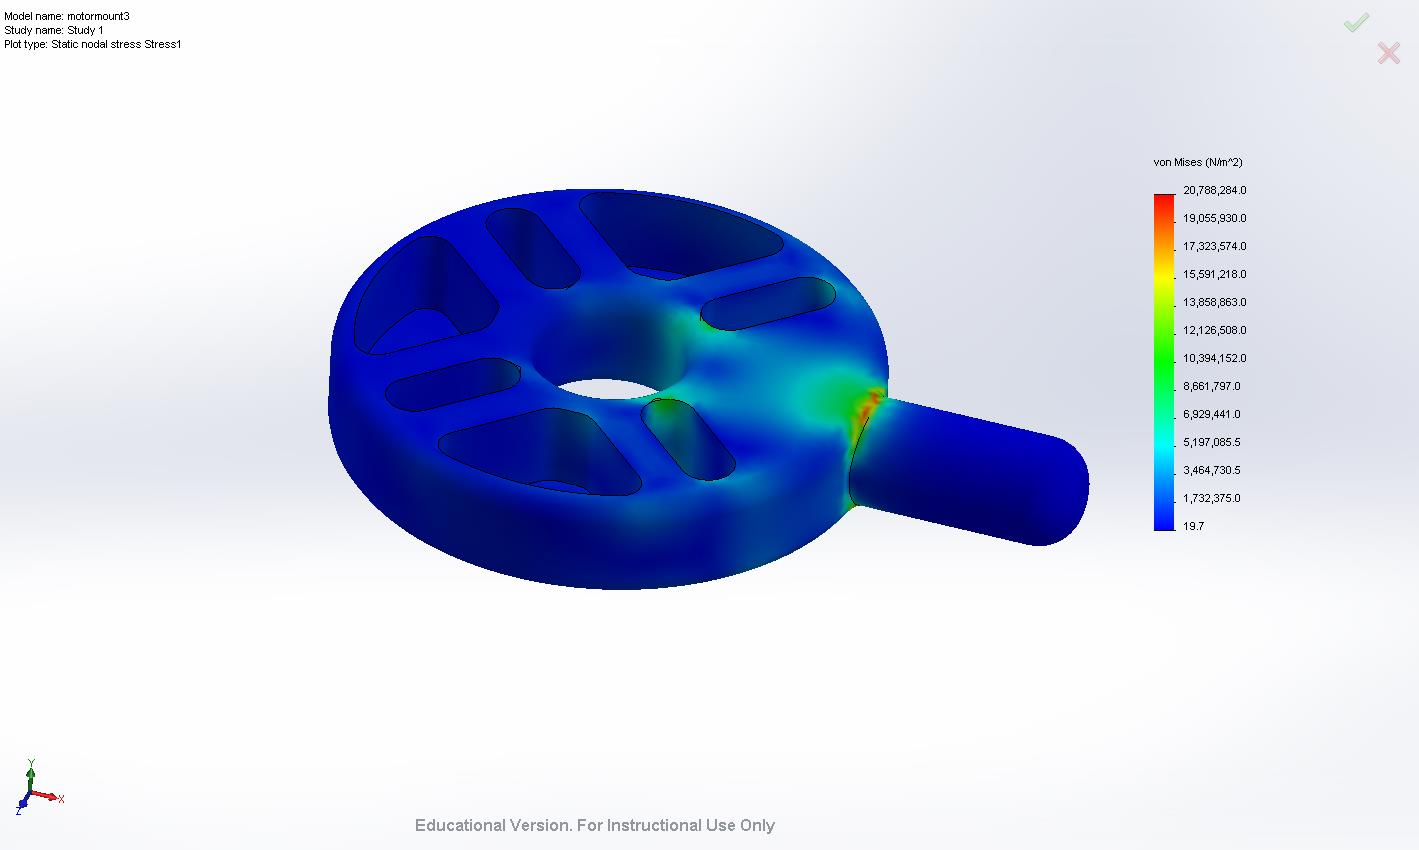
\includegraphics[width=0.6\textwidth]{img/fea_stress.jpg}
	\caption{FEA with red indicating high levels of stress. Forces applied
	perpendicular to flat mount.}
	\label{fig:feastress}
\end{figure}
 
\begin{figure}[!h]
	\centering
	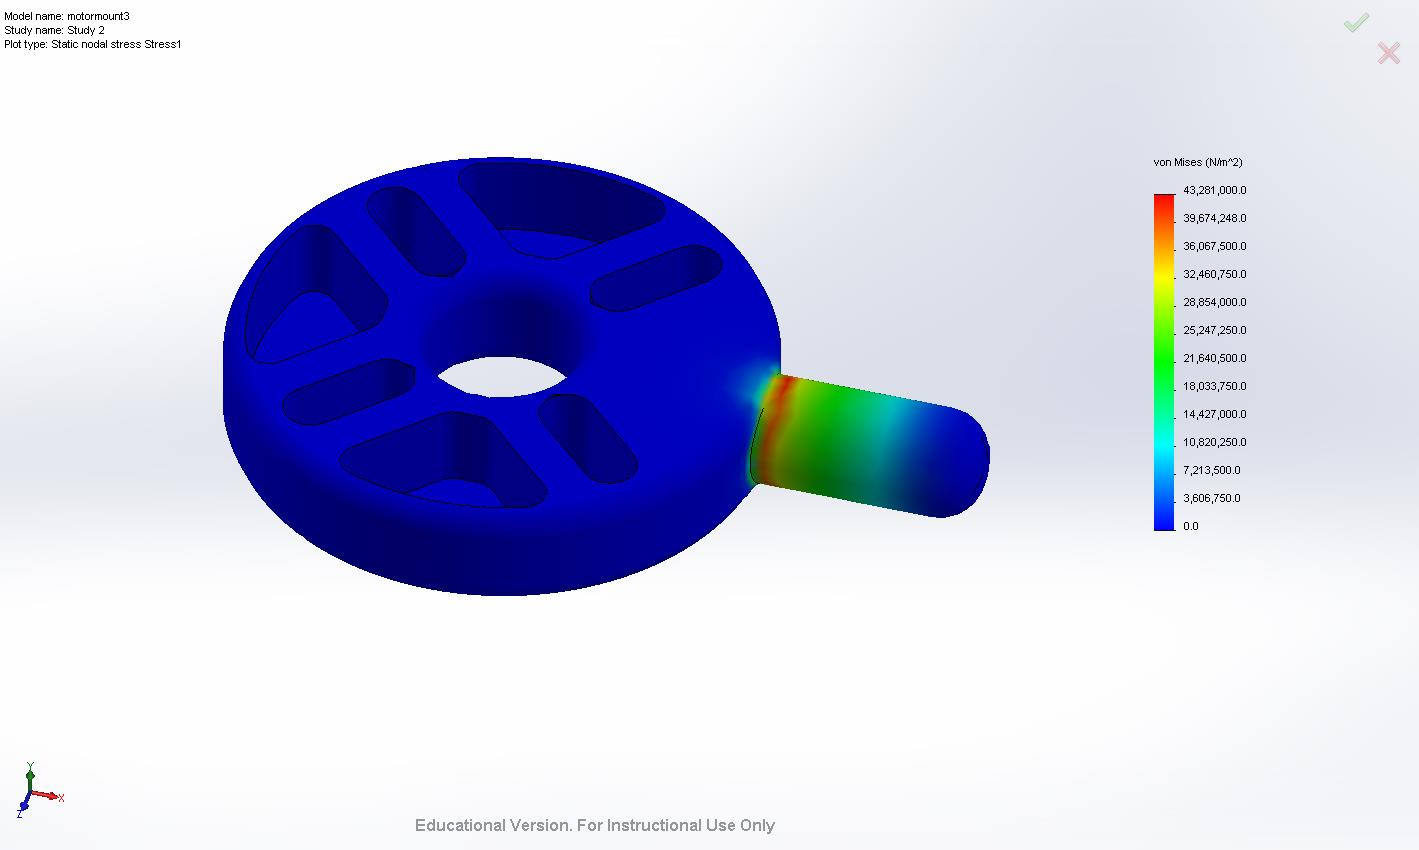
\includegraphics[width=0.6\textwidth]{img/fea_strain.jpg}
	\caption{FEA with red indicating high levels of stress. Forces applied
	torsionally simulating torques from Figure~\ref{fig:mmi}.}
	\label{fig:feastrain}
\end{figure}

\begin{figure}[!h]
	\centering
	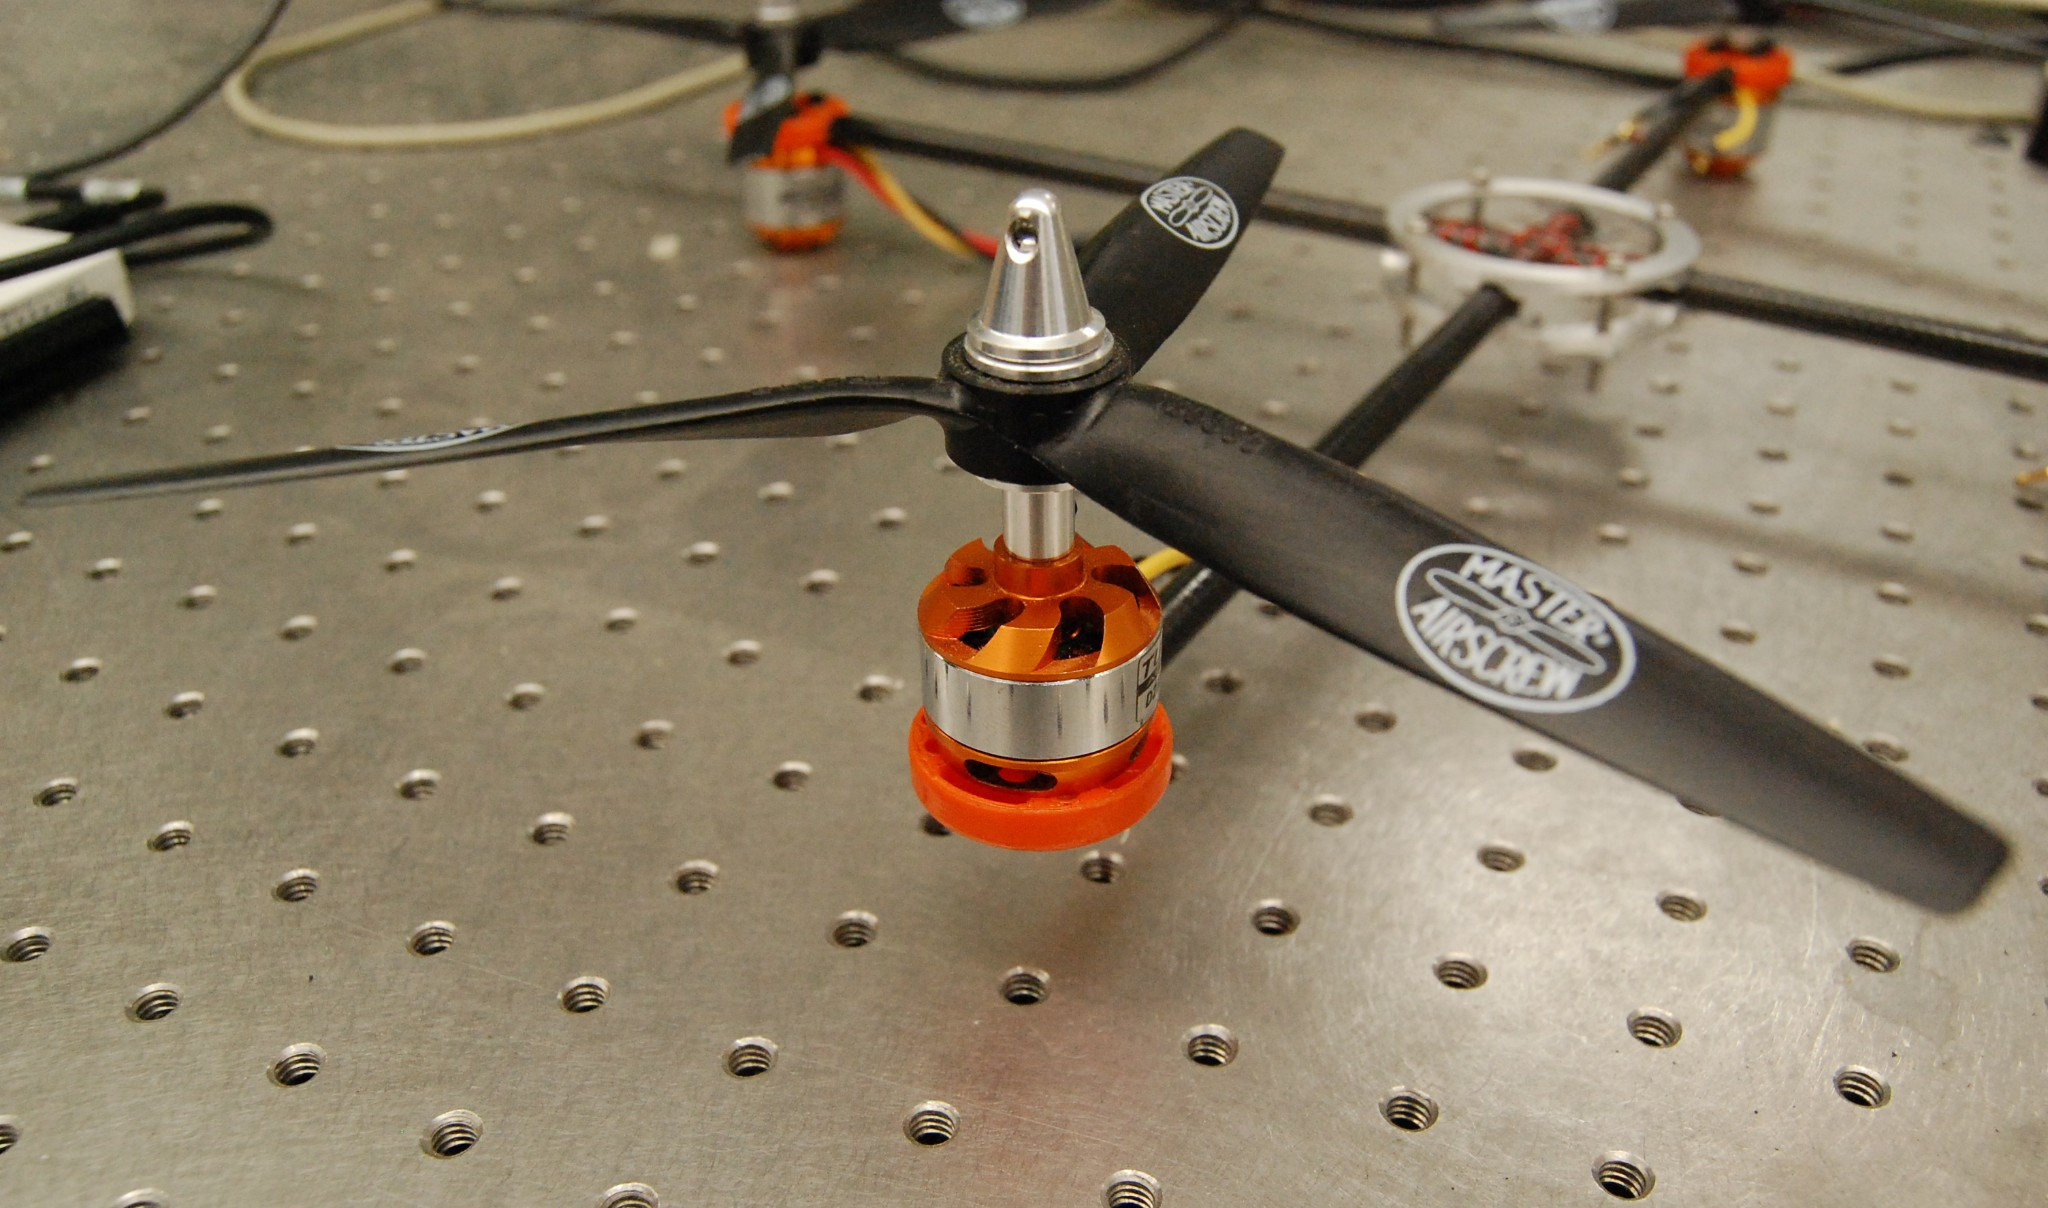
\includegraphics[width=0.6\textwidth]{img/motor_mount_initial.jpg}
	\caption{Initial motor mount configuration. The longer moment arm made the
	mount prone to vibrations.}
	\label{fig:mmi}
\end{figure}

\begin{figure}[!h]
	\centering
	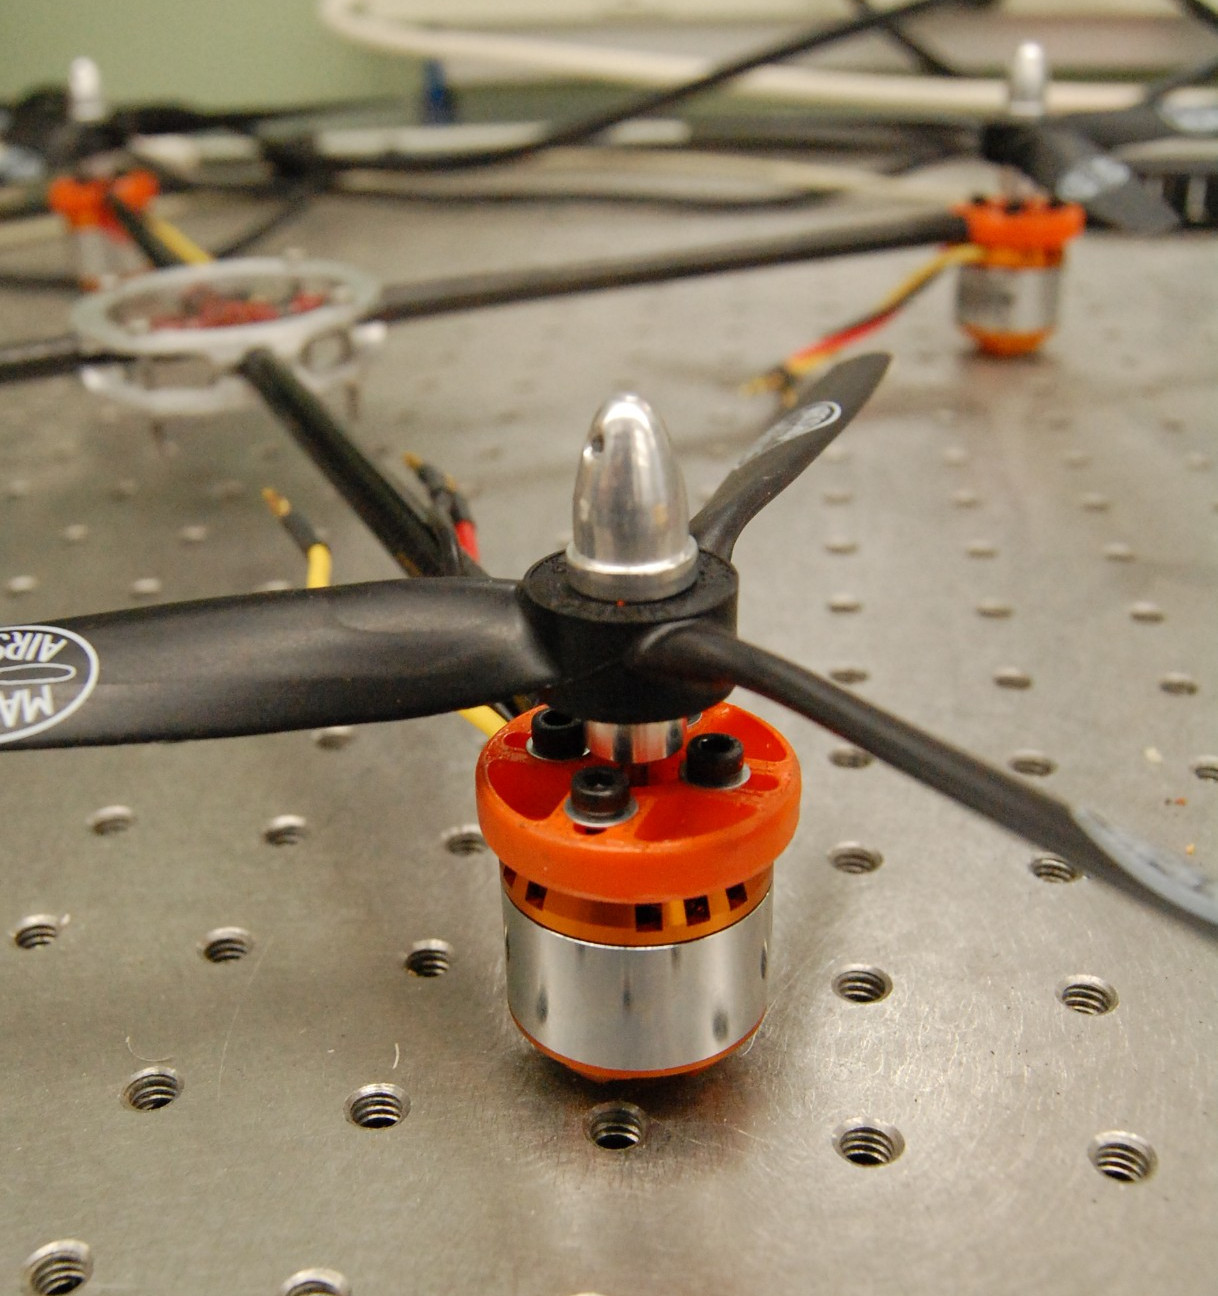
\includegraphics[width=0.5\textwidth]{img/motor_mount_final.jpg}
	\caption{Final motor mount configuration. Having the two rotating masses on
	either side of the mount reduces vibration.}
	\label{fig:mmf}
\end{figure}

\begin{figure}[!h]
	\centering
	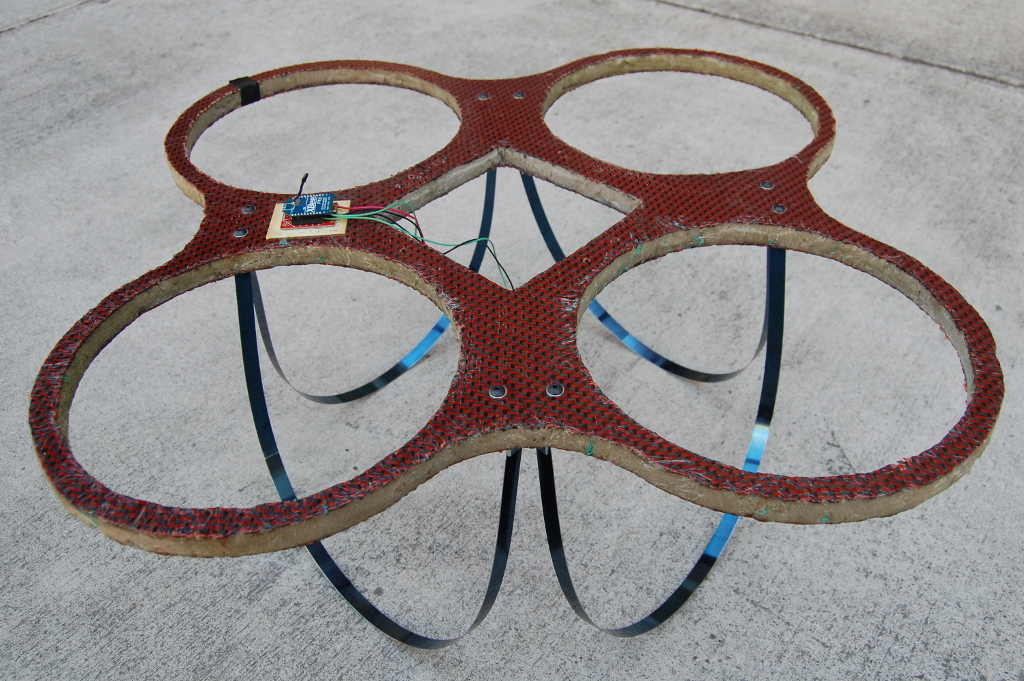
\includegraphics[width=0.6\textwidth]{img/prop_guard.jpg}
	\caption{Propeller guard with landing gear mounted.}
	\label{fig:feastress}
\end{figure}


\section*{Electronics}

\subsection*{Power}

All electronics on the quadrotor are powered by two 4S 1000 mAh lithium polymer
batteries wired in parallel. While using a single 2000 mAh battery would have
been ideal, we were unable to find such a battery with the desired dimensions.

Four Turnigy D2830-11 1000kv brushless motors powered by Turnigy Plush 18A ESCs
turning 8x6 Master Airscrew 3-blade propellers provide us with our performance
characteristic of 50\% throttle hover.

The Texas Instruments PTN78020WAH wide-input voltage-adjustable switching
regulator provides steady 5V power at up to 6A for onboard logic and small
actuators. The regulator is integrated into our flight control board and also
powers a linear regulator that in turn supports a 3.3V logic bus.


\subsection*{Onboard Computing: Odroid-X2}

In 2012, many teams, including our own, were wracked by wireless interference
due to overusage of the 2.4 GHz band in the competition arena. We decided to
work around this issue by confining all computation to the quadrotor itself,
with only a 900 MHz downlink for killswitch activation.

The Odroid-X2 is a 4''-square mini-PC built around the Samsung Exynos 4412
quad-core processor clocked at 2 GHz (Figure~\ref{fig:odroids}). Each
quadrotor is built with a single Odroid onboard. In 2013 we planned to use two
Odroids due to the demanding computational task of processing a 3D map, but the
2014 mission presents a much simpler computational task for which only a single
Odroid is needed.

\begin{figure}[!h]
	\centering
	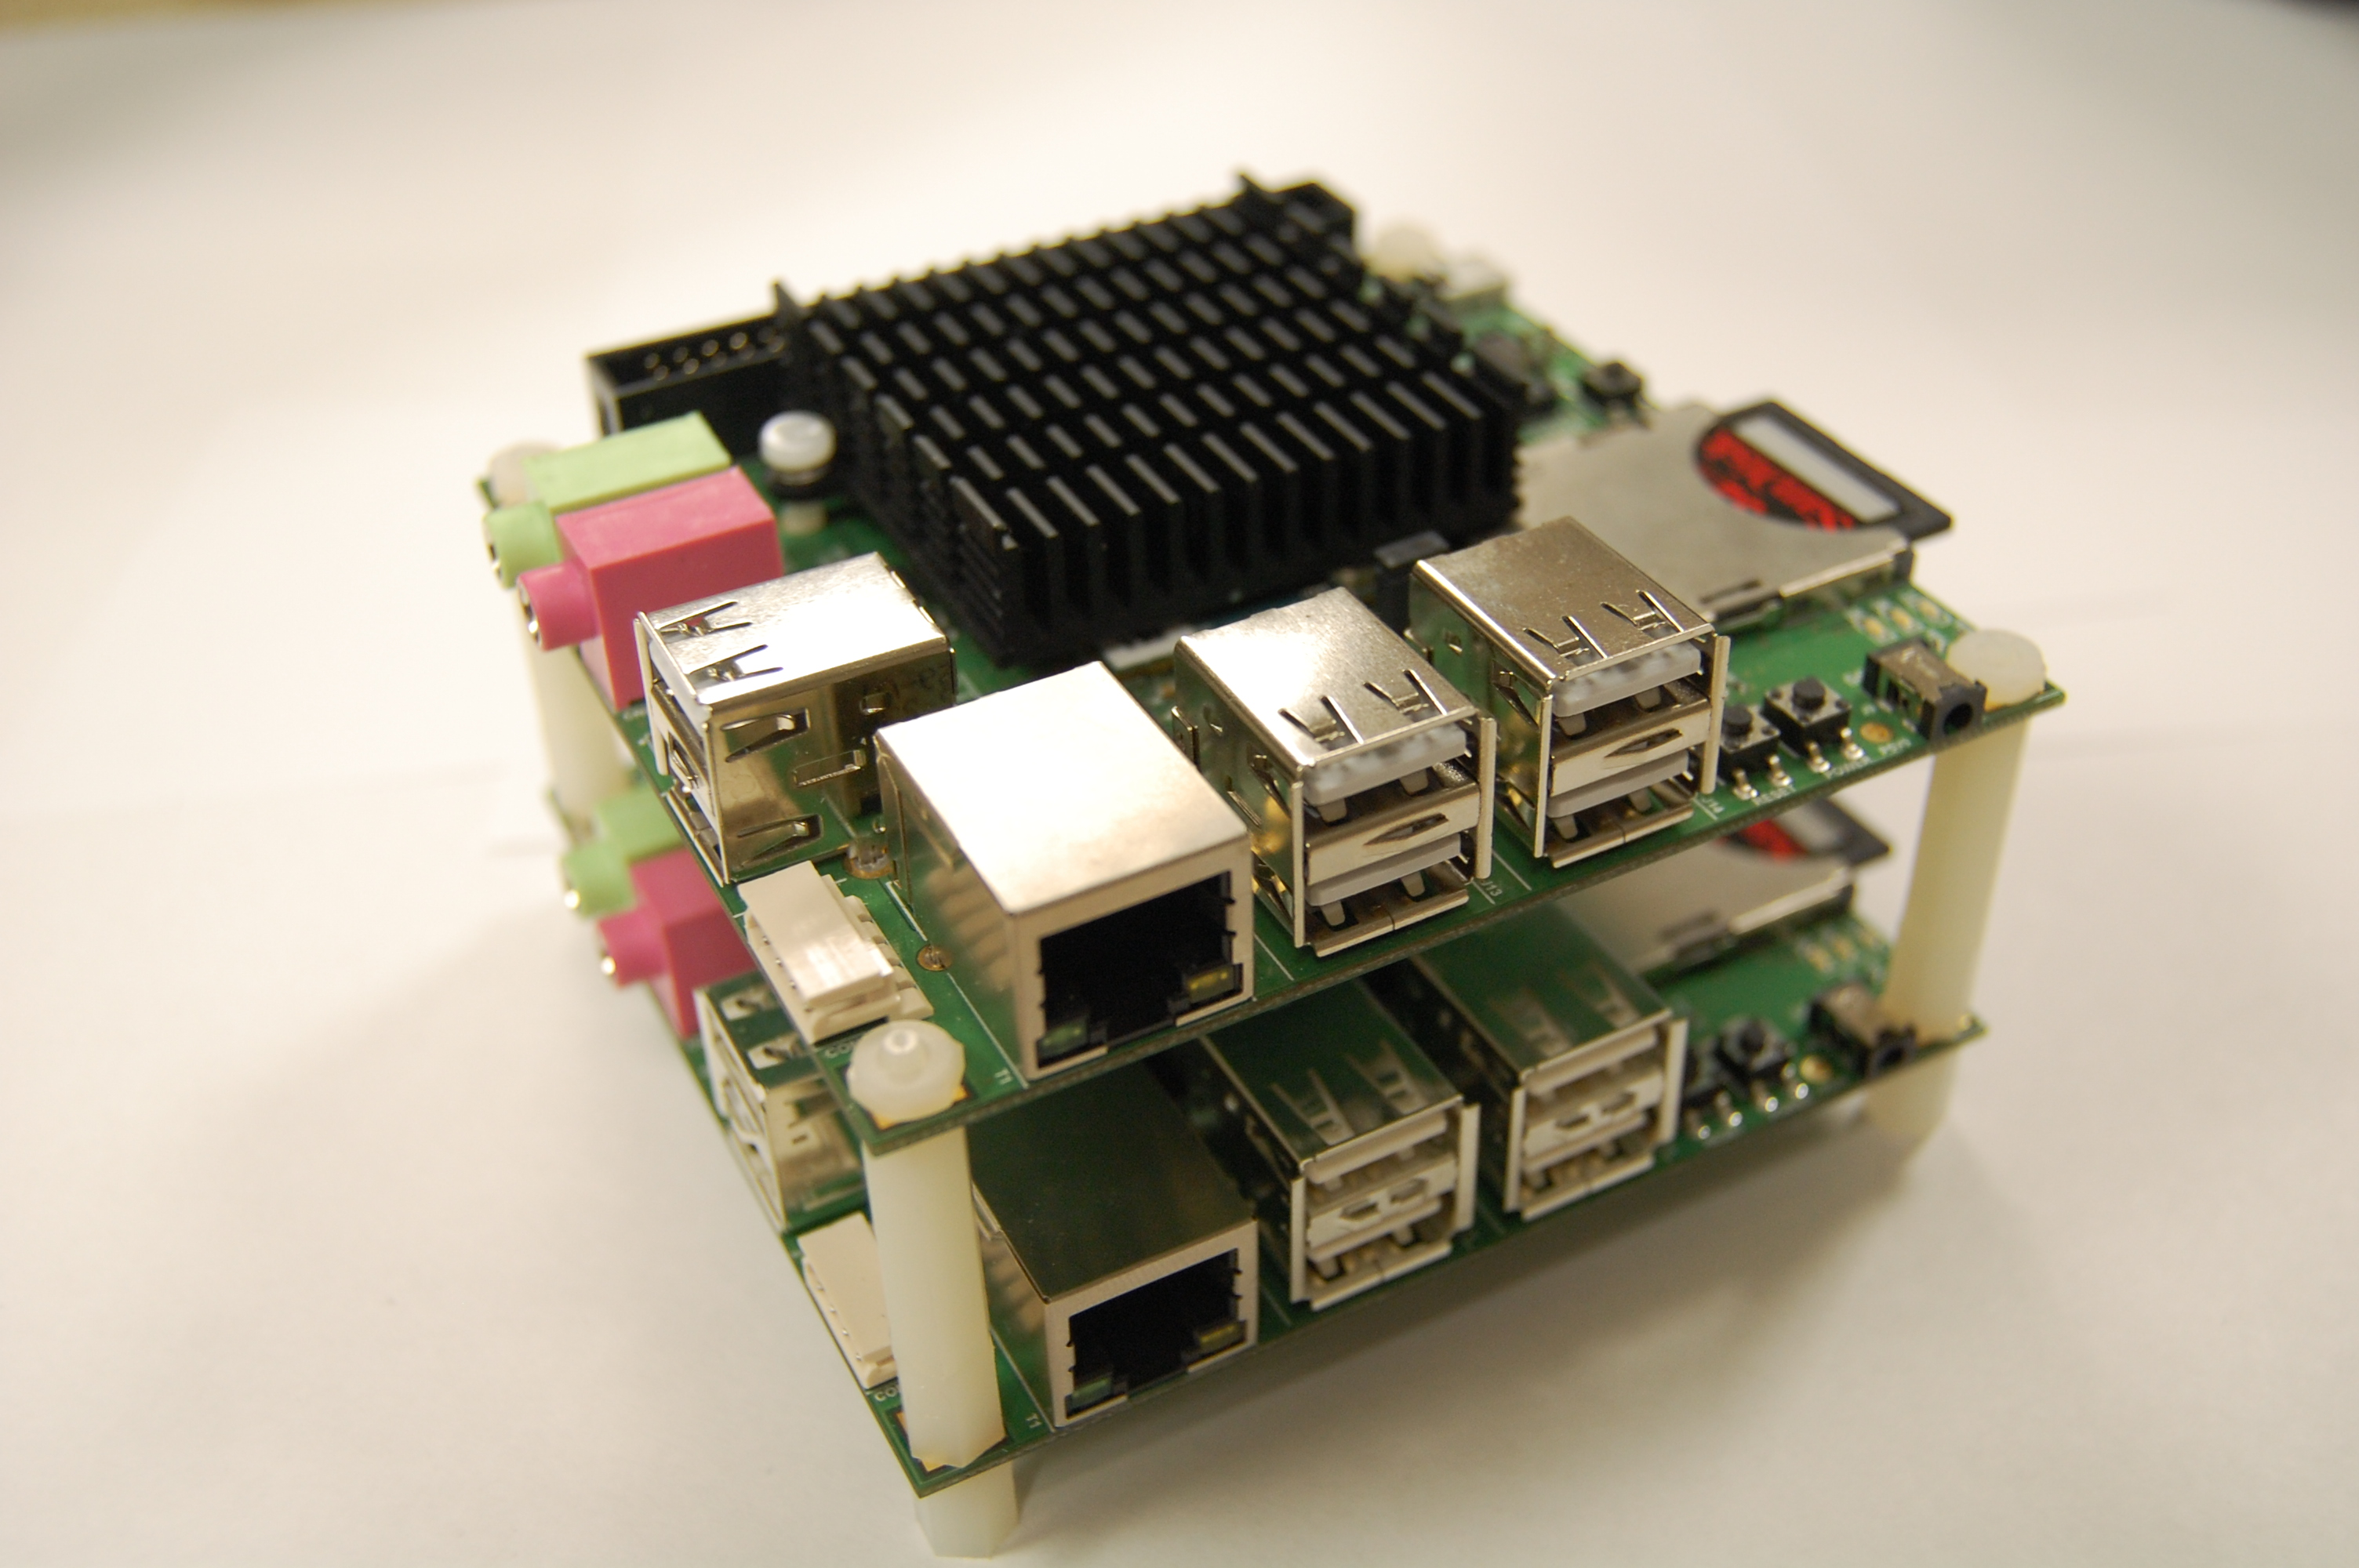
\includegraphics[width=0.6\textwidth]{img/odroid_stack.jpg}
	\caption{Stack of two Odroids.}
	\label{fig:odroids}
\end{figure}


\subsection*{Localization: Pixhawk PX4Flow}

The PX4Flow is an optical flow camera capable of processing images at 752x480
at up to 250 Hz. It operates in much the same way as a modern optical mouse
sensor, comparing subsequent video frames to measure motion. It features an
onboard sonar sensor coupled with an IMU to measure vehicle altitude while
accounting for tilt.

The data from the PX4Flow is sent to the flight control board, which fuses the
measurement with other sensor data to determine the quadrotor's current
location. It then uses navigation data from the Odroid to plan a path to the
desired position.

% TODO: Picture of PX4Flow
\begin{figure}[!h]
	\centering
	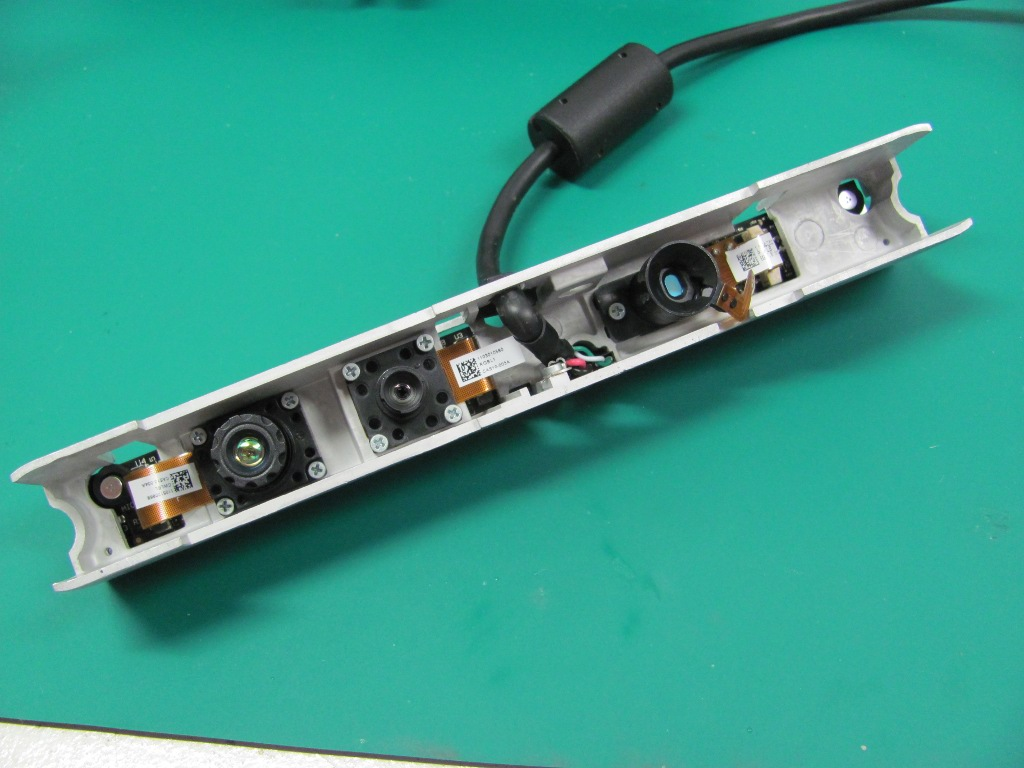
\includegraphics[width=0.6\textwidth]{img/xtion.jpg}
	\caption{ASUS Xtion Pro Live without external housing.}
	\label{fig:xtion}
\end{figure}


\subsection*{Flight Control Board (STM32F405)}

The 2012 flight control board built around the ATXmega128a3, while sufficient
for basic flight, was scrapped in favor of using the much more powerful
STM32F405 in order to achieve 1 kHz flight stabilization. Although we do not
yet take full advantage of this higher control loop frequency, it effects lower
gyroscopic drift and allows for higher PID gains and tighter control.

\begin{figure}[!h]
	\centering
	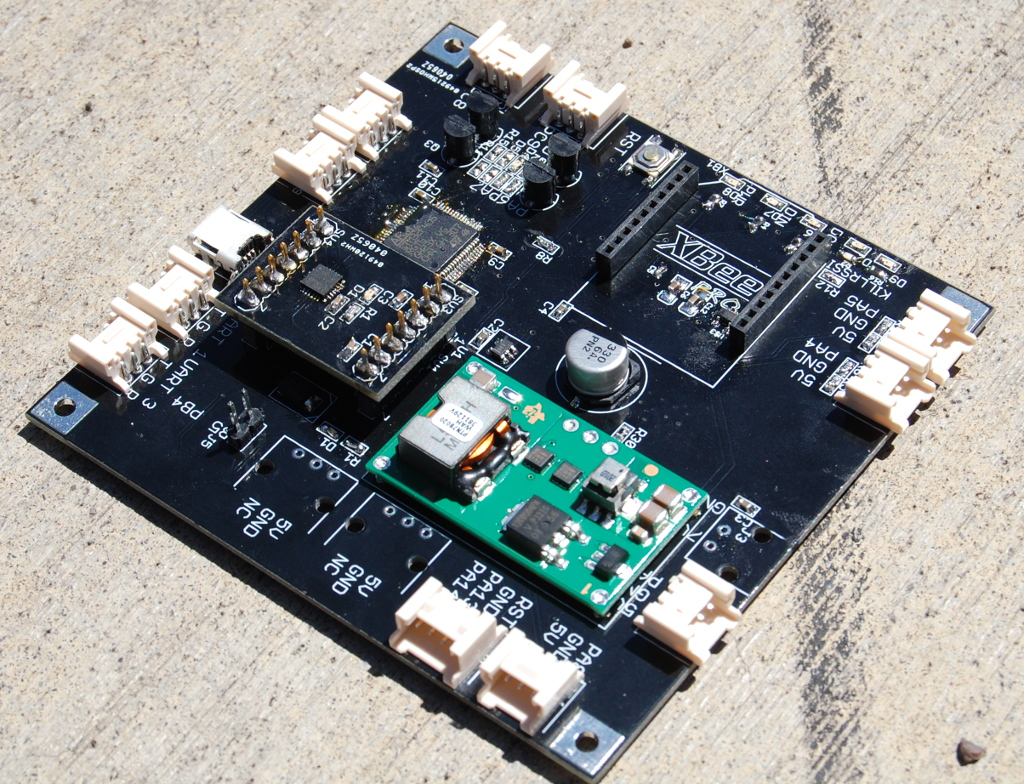
\includegraphics[width=0.6\textwidth]{img/flight_control.jpg}
	\caption{The latest revision of the flight control board.}
	\label{fig:fcboard}
\end{figure}

The flight control board controls four ESCs with 400 Hz PWM signals and has
four SPI connectors available for future use of a custom 1 kHz-capable,
SPI-enabled ESC. The flight control board receives flight commands from either:

\begin{itemize}
	\item The Odroid over a 460800 baud USART bus for autonomous control, or
	\item The XBee over a 38400 baud USART bus for manual control.
\end{itemize}

Orientation estimates are calculated using feedback from an InvenSense MPU-6000
six-axis gyroscope/accelerometer chip, which is polled at 1 kHz in sync with
the flight control loop. In order to best isolate the IMU from chassis
vibrations and to mitigate sensor drift caused by board flex, it is mounted on
a separate board above the rest of the flight control board.


\subsection*{Killswitch and Wireless Communication}

The killswitch is located between the STM32F405 and the ESCs. The signal
required to keep the killswitch closed is generated by a 900 MHz XBee Pro and is
not associated with the flight control software at all. The killswitch must be
armed for the ESCs to receive any signal from the STM32F405.

The onboard XBee is paired with another XBee held by a human operator. A pair
of pins between the two XBees are configured to mirror each other such that the
state of the pin on both XBees can be changed by a switch held by the operator.
This minimizes the amount of software and electronics involved, thereby
maximizing reliability.


\section*{Software}

The Odroid will run software to detect ground robots, make high-level
decisions, and perform high-level obstacle avoidance and path planning. Flight
commands will be sent to the flight control board, which maintains the
quadrotor at the desired orientation with a 1 kHz control loop.


\subsection*{Robot Operating System}

Robot Operating System (ROS) is a collection of libraries and tools that allows
developers from around the world to contribute software packages such as device
drivers, messaging libraries, and visualizers in a consistent format for others
to use.

We have developed our high-level control systems to operate within this
software architecture. This allows us to use third-party joystick drivers, path
planning libraries, and general purpose algorithms, which frees us from having
to reimplement solved problems.

In addition, due to ROS's exclusive use of TCP/UDP network protocols for
inter-process communication, we can easily debug live data from a remote base
station over a network.


\subsection*{Ground Robot Detection}

We will design a vision system that is able to detect both ground robots and
obstacle robots. This vision system will need to have predictive capabilities
for when robots are outside the camera's frame. Due to the requirement of a lens
with a very short focal length, the software will need to rectify the image so
as to not interpret lens distortion as robot motion. Due to the angular motion
of the quadrotor, the software will need to be aware of the vehicle's current
orientation to maintain the locations of ground robots in a global frame.


\subsection*{Strategy Algorithm}

The robot location data needs to be processed to determine what action the
quadrotor should take. The strategy software will factor in the quadrotor's
location, the ground robots' locations and directions of travel, and the
current state of the playing field to make an intelligent decision.

Through our competition simulator, we have found a simple algorithm that
produces good results. The highest priority goal is to keep robots from leaving
the arena, so the quadrotor should always attempt to change the direction of
those robots closest to the white or red edges of the field. It can then work
its way inward to lower priority robots.


\subsection*{Flight Control}

In order to mitigate the added complexity of the STM32F4 over the ATXmega128
used on our 2012 quadrotor, we write our controllers as processes within
ChibiOS, a real-time operating system for embedded devices. ChibiOS provides
basic functionality for managing threads, mutexes, and a hardware abstraction
layer. We run two main threads: a 1 kHz flight control loop and a 100 Hz
communications loop. Since these threads are created in the same generic format
such as the following control loop thread, we can easily add more processes:

\begin{center} \begin{minipage}{5.5in}

{\scriptsize

\begin{verbatim}
/*
 * Control loop
 */
static WORKING_AREA(wa_control_thread, 128);
static msg_t control_thread(void *arg)
{
    (void) arg;
    chRegSetThreadName("control");

    systime_t time = chTimeNow();

    /* DCM of body in global frame. */
    float dcm_bg[3][3];
    m_init_identity(dcm_bg);

    /* Motor duty cycles */
    float motor_dc[4];

    while (TRUE) {
        time += MS2ST(CONTROL_DT*1000);   // Next deadline in 1 ms.

        update_ahrs(CONTROL_DT, dcm_bg);
        run_controller(dcm_bg, motor_dc);
        update_motors(motor_dc);

        chThdSleepUntil(time);
    }

    return 0;
}
\end{verbatim}

}

\end{minipage} \end{center}

The 1 kHz control loop stabilizes the quadrotor in the air by doing the
following in succession:

\begin{enumerate}
	\item Read IMU (gyroscope and accelerometer)
	\item Update orientation estimate
	\item Run cascading PID controllers on current and desired orientations
	\item Update ESC duty cycles appropriately
\end{enumerate}

This code was largely ported over from code used in our 2012 tricopter (built
experimentally, not used for competition). The higher loop frequency lends
improved stability and reduced gyroscopic drift, thus making higher-speed
maneuvers feasible.


\section*{Testing and Safety}

\subsection*{Competition Simulator}

To gain a better understanding of the Mission 7 rules, we created a competition
simulator that simulates the ground robot and obstacle robot behavior
(Figure~\ref{fig:iarc_sim}). This allows us to prototype our ground robot
selection and path planning algorithms quickly without the need for hardware.

\begin{figure}[!h]
	\centering
	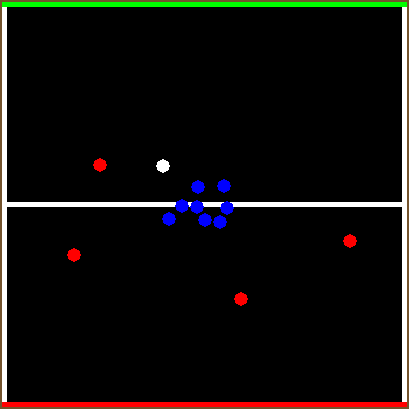
\includegraphics[width=0.6\textwidth]{img/iarc_sim.png}
	\caption{Competition simulator.}
	\label{fig:iarc_sim}
\end{figure}

\subsection*{Table Mount}

A restrictive three-dimensional arm was built to safely test and demonstrate
the quadrotor (Figure~\ref{fig:quad_test_mount}). The arm limits the
quadrotor's ability to move. This was developed in response to previous crash
tests that resulted in hours of wasted time fixing broken hardware.

\begin{figure}[!h]
	\centering
	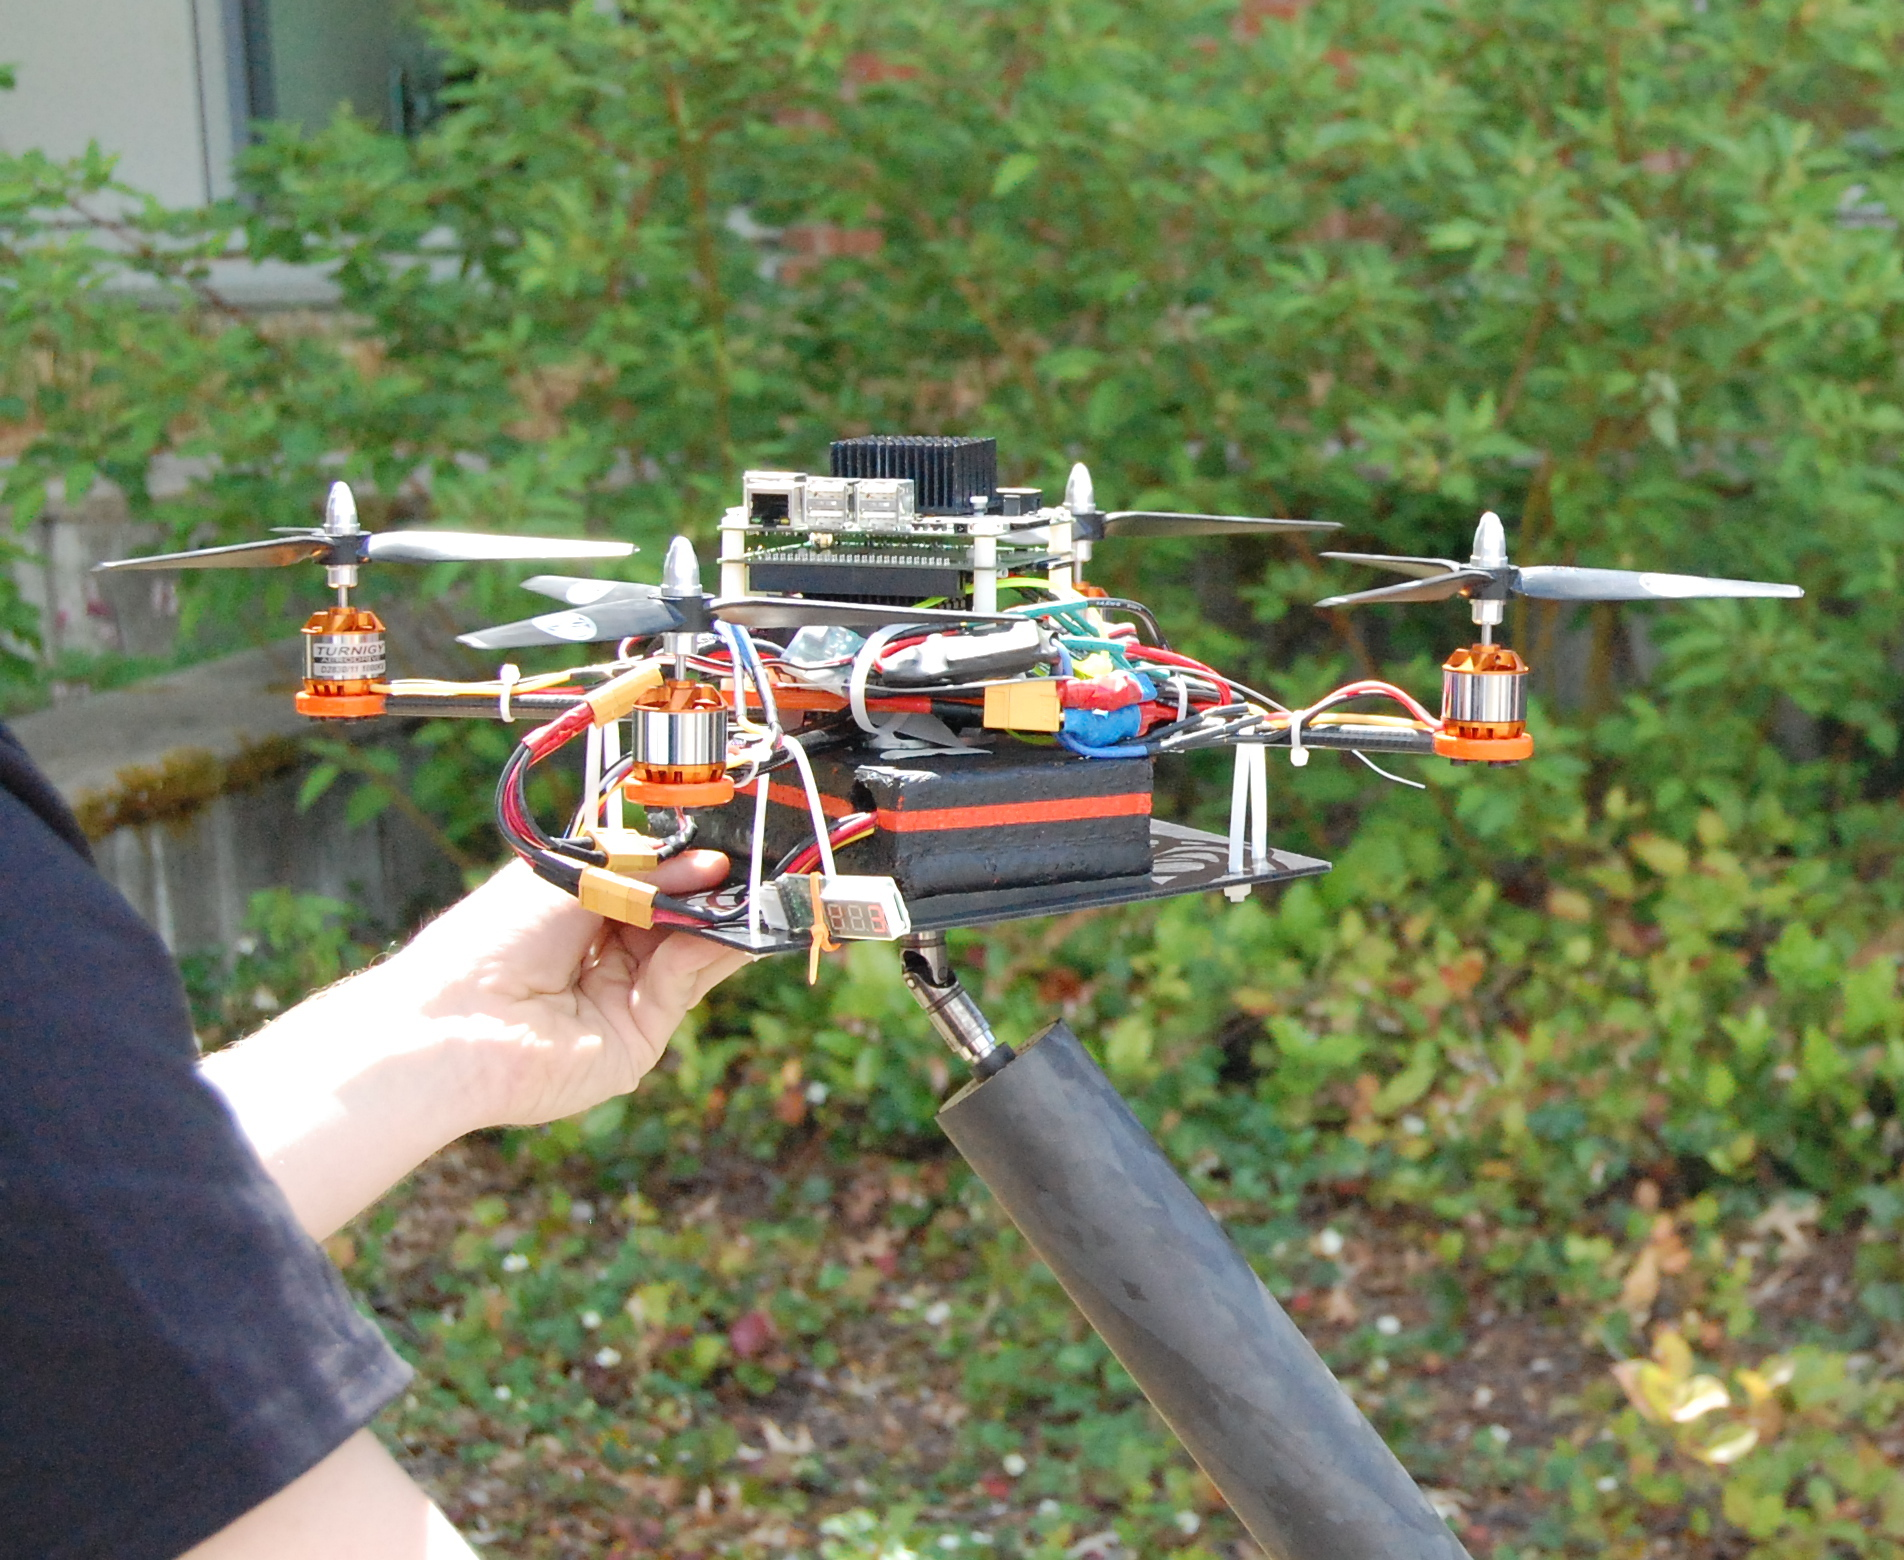
\includegraphics[width=0.6\textwidth]{img/quad_test_mount.jpg}
	\caption{Quadrotor on test mount.}
	\label{fig:quad_test_mount}
\end{figure}

Several design solutions were explored culminating in the current telescoping
arm design. One such alternative was a C-shape frame structure, with a pulley
system that was able to move the quadrotor horizontally and vertically. This
idea was deemed impractical due to its unwieldy size and weight.

Our final design is capable of being collapsed when not in use and extended
during testing. The arm, when clamped to a table, is able to rotate 360 degrees
and provides the quadrotor with a freedom of motion 4 feet in diameter and
2 feet in height. The test stand helps prevent catastrophic damage to the
quadrotor during testing.


\section*{Conclusion}

The OSU Autonomous Aerial Robotics Team has constructed an ambitious entry to
the Mission 7 challenge. With custom flight control breakout board, onboard
processing for vision and navigation, a lightweight chassis for longer
flight time, comprehensive safety features, the quadrotor is a completely
autonomous and untethered flying machine.

Porting over flight control software to the real time operating system ChibiOS
allowed us to take advantage of the ARM processor and its capability to
multithread.

Optimizing the chassis to meet competition requirements gave us new challenges.
We applied root cause failure analysis to determine vibrations were caused by
long moment arms from the propellers. In addition we developed a way to safely
perform full flight tests without fear of damaging the quadrotor.

Developing a solution to radio interference problems introduced the hurdle of
onboard processing. Access to sufficient processing power is perhaps the
biggest challenge of this year and has led to much of the software design
choices.

We will measure our success at the 2014 competition by our ability to maintain
flight for the full competition time, avoid obstacle robots, and herd a few
ground robots to the goal.

Next year we will concentrate on Mission 7b and explore strategies for avoiding
and cooperating with other aerial vehicles.


\section*{Thank You}

We would like to thank the OSU College of Engineering, DW Fritz Automation, and
the National Science Foundation for their generous support.

\end{document}
